%=====================================================================
%  EVALUACIÓN UNIDAD IV — INGENIERÍA DE REQUISITOS (ISR-401)
%  Universidad Técnica Estatal de Quevedo
%  Compilación:  pdflatex Villafuerte_Allan_Unidad4.tex   (x2)
%=====================================================================
\documentclass[12pt,letterpaper]{article}

\usepackage[utf8]{inputenc}
\usepackage[T1]{fontenc}
\usepackage[spanish,es-tabla,es-noquoting]{babel}
\usepackage{mathptmx}                 % Times New Roman
\usepackage[margin=2.5cm]{geometry}
\usepackage{graphicx}
\usepackage{array}
\usepackage{longtable}
\usepackage{ragged2e}
\usepackage{enumitem}
\usepackage{caption}
\usepackage{float}
\usepackage{fancyhdr}
\usepackage[hidelinks]{hyperref}
\usepackage{tikz}
\usetikzlibrary{shapes.geometric,shapes.multipart,shapes.misc,arrows.meta,
                positioning,calc,fit,backgrounds}

\setlength{\parindent}{0pt}
\setlength{\parskip}{6pt}
\justifying
\renewcommand{\arraystretch}{1.25}
\captionsetup{font=small,labelfont=bf}

\pagestyle{fancy}
\fancyhf{}
\fancyhead[L]{\small Ingeniería de Requisitos --- Unidad IV}
\fancyhead[R]{\small Villafuerte Rosero Allan Noe}
\fancyfoot[C]{\small\thepage}
\renewcommand{\headrulewidth}{0.4pt}

%---------------------------------------------------------------------
%  ESTILOS TikZ
%---------------------------------------------------------------------
\tikzset{
  clase/.style={
    rectangle split, rectangle split parts=3, draw, thick,
    rectangle split part align=left, text width=4.1cm,
    align=left, font=\scriptsize, inner sep=4pt},
  actividad/.style={
    rounded rectangle, draw, thick, align=center,
    font=\scriptsize, minimum height=8mm, inner xsep=6pt},
  decision/.style={
    diamond, draw, thick, aspect=2, align=center,
    font=\scriptsize, inner sep=1pt},
  estado/.style={
    rectangle, rounded corners=6pt, draw, thick, align=center,
    font=\scriptsize, minimum height=9mm, minimum width=2.3cm},
  estadoint/.style={
    rectangle split, rectangle split parts=2, rounded corners=6pt,
    draw, thick, align=center, font=\scriptsize, text width=3.1cm,
    inner sep=4pt},
  inicial/.style={circle, fill=black, minimum size=5pt, inner sep=0pt},
  flecha/.style={-{Stealth[length=5pt]}, thick},
  etiq/.style={font=\scriptsize, midway}
}

\begin{document}

%=====================================================================
%  CARÁTULA
%=====================================================================
\begin{titlepage}
\thispagestyle{empty}
\centering

\vspace*{1.2cm}

{\LARGE\bfseries UNIVERSIDAD TÉCNICA ESTATAL DE QUEVEDO\par}

\vspace{0.6cm}

{\Large FACULTAD DE CIENCIAS DE LA COMPUTACIÓN\par}

\vspace{1.4cm}

\rule{\linewidth}{0.6pt}

\vspace{0.8cm}

{\Large\bfseries EVALUACIÓN UNIDAD IV\par}

\vspace{0.5cm}

{\large Modelado de Sistemas, Especificación, Validación\\
y Gestión de Requisitos\par}

\vspace{0.8cm}

\rule{\linewidth}{0.6pt}

\vspace{1.8cm}
\begin{center} 
 \textbf{Asignatura:} Ingeniería de Requisitos \\
 \textbf{Alumno:} Villafuerte Rosero Allan Noe \\
 \textbf{Curso:}  4to Software ``A'' \\
 \textbf{Docente:}  Ing. Guerrero Ulloa Gleiston Cicerón\\ 
 \textbf{Repositorio:} \\\url{https://github.com/AlanNVR/Villafuerte_Allan}
\end{center}
\vfill

{\large Quevedo --- Los Ríos --- Ecuador\par}
\vspace{0.3cm}
{\large 11 de agosto de 2026\par}

\end{titlepage}

%=====================================================================
%  PÁGINA DE CAPTURAS
%=====================================================================
\section*{Capturas del cuestionario (SGA)}
\addcontentsline{toc}{section}{Capturas del cuestionario (SGA)}

\begin{figure}[H]
\centering
\fbox{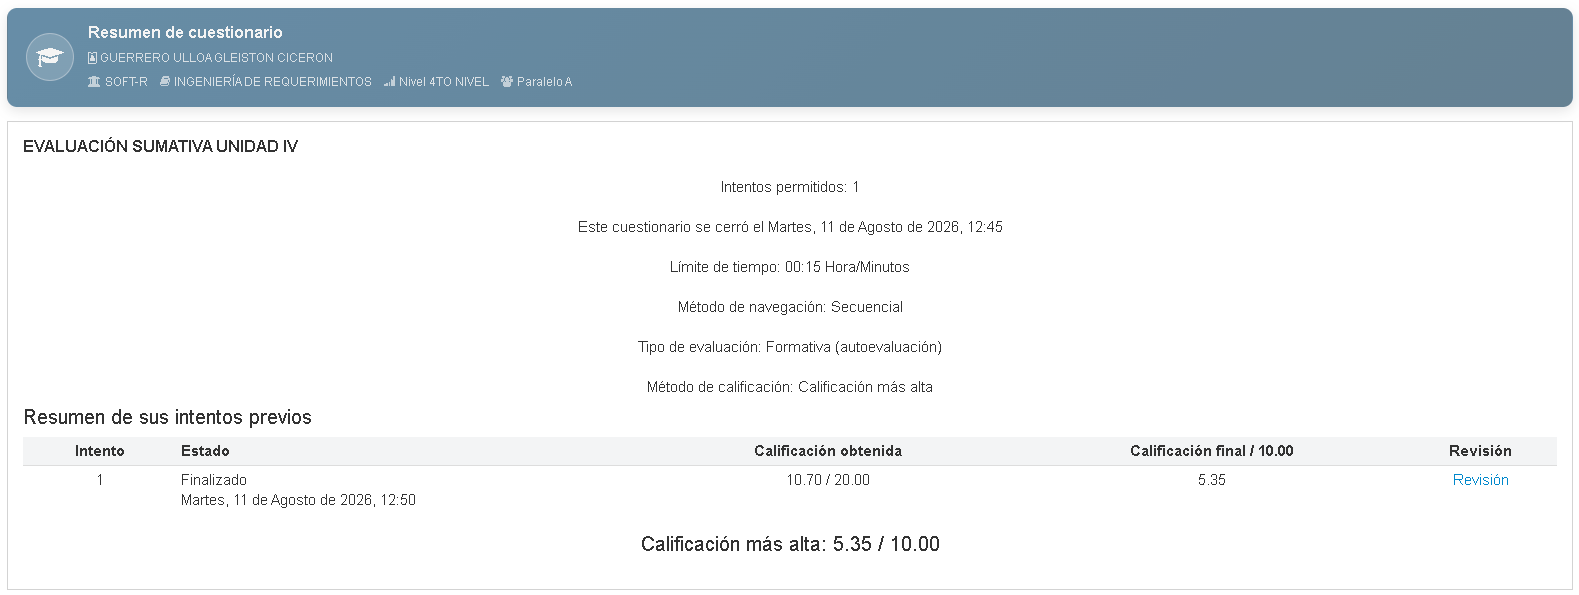
\includegraphics[width=0.95\linewidth]{Figuras/Imagen1.png}}
\caption{Resumen del cuestionario --- Evaluación Sumativa Unidad IV.}
\label{fig:resumen}
\end{figure}

\vspace{0.6cm}

\begin{figure}[H]
\centering
\fbox{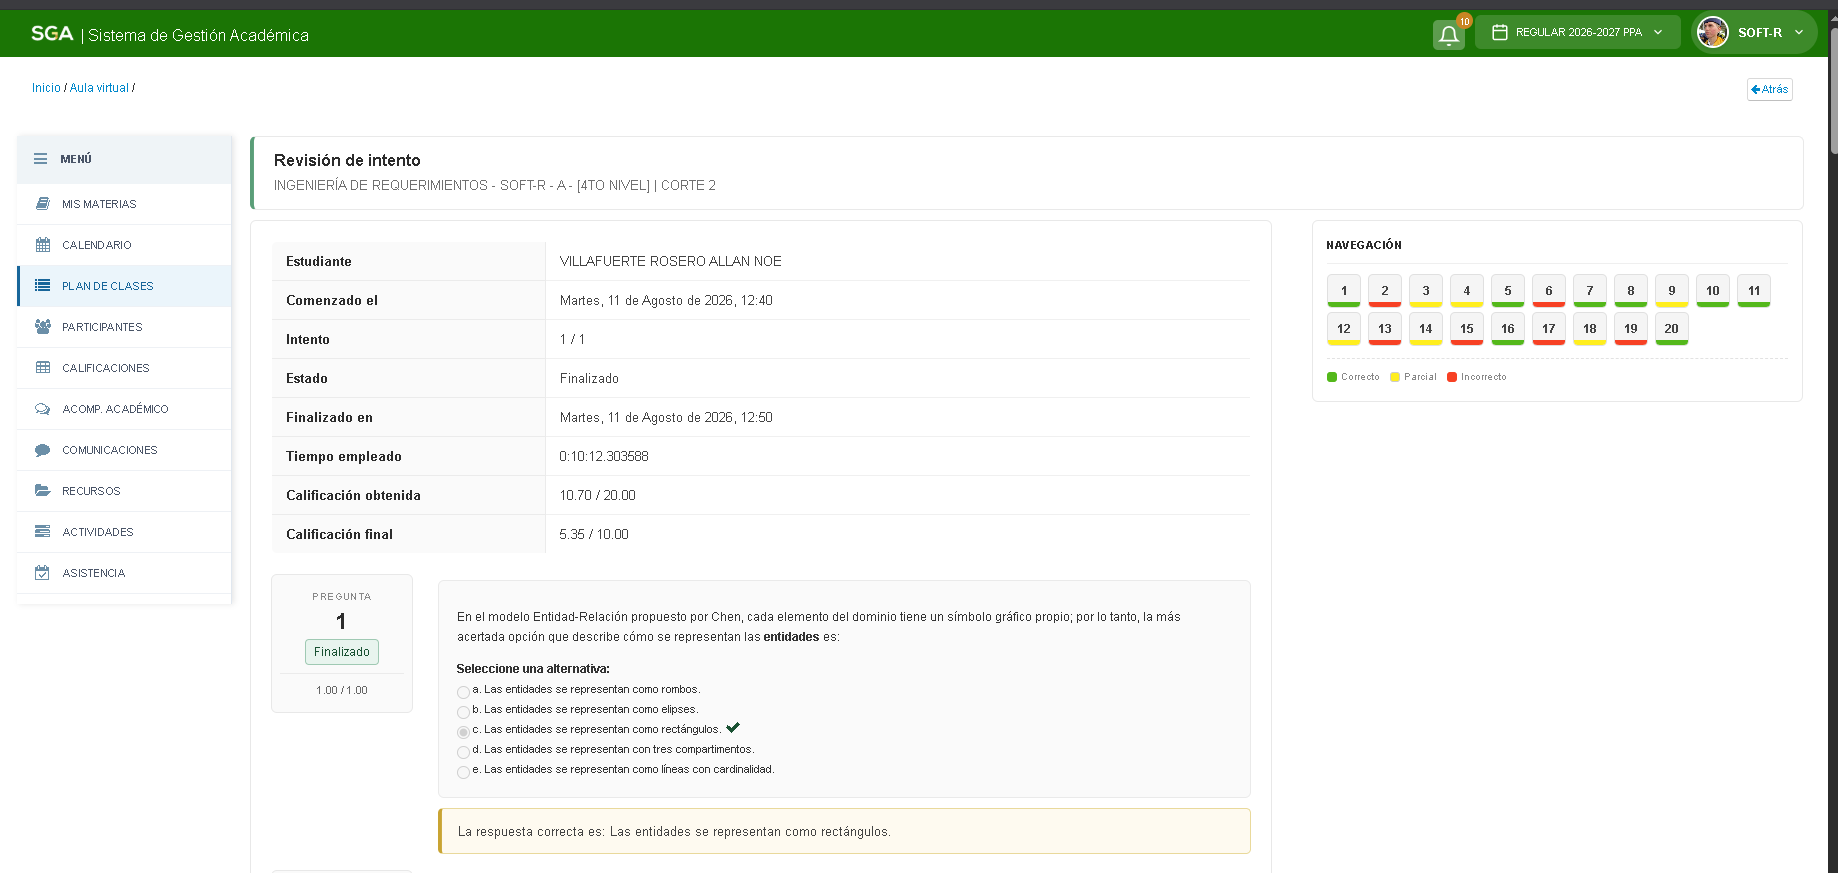
\includegraphics[width=0.95\linewidth]{Figuras/Imagen2.png}}
\caption{Revisión del intento realizado en el Sistema de Gestión Académica.}
\label{fig:revision}
\end{figure}

\clearpage

%=====================================================================
%  P1
%=====================================================================
\section*{P1. Modelo de datos --- Diagrama de clases UML}

\begin{figure}[H]
\centering
\scalebox{0.92}{
\begin{tikzpicture}[node distance=1.8cm]

\node[clase] (cliente) {
  \textbf{Cliente}
  \nodepart{two}
    -- cédulaRUC: String \{id\}\\
    -- nombre: String\\
    -- correo: String\\
    -- teléfono: String
  \nodepart{three}
    + registrarPedido()
};

\node[clase, right=3.2cm of cliente] (pedido) {
  \textbf{Pedido}
  \nodepart{two}
    -- idPedido: String \{id\}\\
    -- fecha: Date\\
    -- total: Decimal\\
    -- estado: String
  \nodepart{three}
    + confirmar()\\
    + despachar()\\
    + entregar()\\
    + anular()\\
    + calcularTotal()
};

\node[clase, below=2.6cm of pedido] (linea) {
  \textbf{LíneaPedido}
  \nodepart{two}
    -- cantidad: int\\
    -- precioUnitario: Decimal\\
    -- subtotal: Decimal
  \nodepart{three}
    + calcularSubtotal()
};

\node[clase, left=3.2cm of linea] (producto) {
  \textbf{Producto}
  \nodepart{two}
    -- código: String \{id\}\\
    -- descripción: String\\
    -- precio: Decimal\\
    -- stock: int
  \nodepart{three}
    + verificarStock()\\
    + descontarStock()
};

% Cliente 1 -- 0..* Pedido
\draw[thick] (cliente.east) -- (pedido.west)
      node[midway,above,font=\scriptsize]{realiza}
      node[pos=0,above right=2pt and 3pt,font=\scriptsize]{1}
      node[pos=1,above left=2pt and 3pt,font=\scriptsize]{0..*};

% Pedido 1 <>-- 1..* LineaPedido (composición)
\draw[thick,{Diamond[fill=black,length=7pt,width=5pt]}-]
      (pedido.south) -- (linea.north)
      node[midway,left,font=\scriptsize]{contiene}
      node[pos=0,below right=6pt and 3pt,font=\scriptsize]{1}
      node[pos=1,above right=2pt and 3pt,font=\scriptsize]{1..*};

% LineaPedido 0..* -- 1 Producto
\draw[thick] (linea.west) -- (producto.east)
      node[midway,above,font=\scriptsize]{referencia}
      node[pos=0,above left=2pt and 3pt,font=\scriptsize]{0..*}
      node[pos=1,above right=2pt and 3pt,font=\scriptsize]{1};

\end{tikzpicture}}
\caption{Diagrama de clases del Sistema de Gestión de Pedidos.}
\label{fig:clases}
\end{figure}


\clearpage

%=====================================================================
%  P2
%=====================================================================
\section*{P2. Modelo funcional --- Diagrama de actividades ``Registrar pedido''}

El flujo incorpora de forma explícita la actividad \textit{Calcular total},
exigida por el RF-01, y organiza las responsabilidades en dos carriles:
\textbf{Cliente} y \textbf{Sistema}.

\begin{figure}[H]
\centering
\scalebox{0.95}{
\begin{tikzpicture}[node distance=0.95cm]

% Carriles
\draw[thick] (-3.7,0.9) rectangle (3.7,-12.2);
\draw[thick] (0,0.9) -- (0,-12.2);
\node[font=\small\bfseries] at (-1.85,0.45) {Cliente};
\node[font=\small\bfseries] at ( 1.85,0.45) {Sistema};
\draw[thick] (-3.7,0.1) -- (3.7,0.1);

\node[inicial] (ini) at (-1.85,-0.7) {};
\node[actividad, below=0.8cm of ini] (recibir) {Recibir solicitud\\de pedido};

\node[actividad] (registrar) at (1.85,-3.3) {Registrar líneas\\del pedido};
\node[actividad, below=of registrar] (total) {Calcular total\\del pedido};
\node[decision, below=of total] (dec) {¿Stock\\disponible?};
\node[actividad, below=1.5cm of dec] (confirmar) {Confirmar pedido\\(estado = Confirmado)};
\node[actividad] (notificar) at (-1.85,-9.15) {Notificar\\faltante};

\coordinate (merge) at (1.85,-10.9);
\node[circle, draw, thick, minimum size=10pt, inner sep=0pt] (fin) at (1.85,-11.6) {};
\node[inicial, minimum size=6pt] at (fin) {};

\draw[flecha] (ini) -- (recibir);
\draw[flecha] (recibir.east) -| (registrar.north);
\draw[flecha] (registrar) -- (total);
\draw[flecha] (total) -- (dec);
\draw[flecha] (dec) -- node[right,font=\scriptsize]{[Sí]} (confirmar);
\draw[flecha] (dec.west) -| node[above,font=\scriptsize,pos=0.25]{[No]} (notificar.north);
\draw[flecha] (confirmar) -- (fin);
\draw[flecha] (notificar.south) |- (merge) -- (fin.west);

\end{tikzpicture}}
\caption{Diagrama de actividades del proceso ``Registrar pedido''.}
\label{fig:actividades}
\end{figure}

\clearpage

%=====================================================================
%  P3
%=====================================================================
\section*{P3. Modelo de comportamiento --- Máquina de estados de \textit{Pedido}}

\begin{figure}[H]
\centering
\scalebox{0.88}{
\begin{tikzpicture}[node distance=1.5cm]

\node[inicial] (ini) {};
\node[estadoint, right=1.2cm of ini] (reg) {
  \textbf{Registrado}
  \nodepart{two}\textit{notificar faltante /}\\\textit{sin cambio de estado}};

\node[estado, right=3.6cm of reg] (conf) {Confirmado};
\node[estado, right=2.2cm of conf] (env)  {Enviado};

\begin{scope}[on background layer]
  \node[draw, thick, dashed, rounded corners=8pt, inner sep=13pt,
        fit=(conf)(env), label={[font=\scriptsize\bfseries,anchor=north west]
        north west:\ Activo}] (activo) {};
\end{scope}

\node[circle, draw, thick, minimum size=13pt, inner sep=0pt,
      right=2.2cm of env, label={[font=\scriptsize]below:Entregado}] (ent) {};
\node[inicial, minimum size=7pt] at (ent) {};

\node[circle, draw, thick, minimum size=13pt, inner sep=0pt,
      below=2.4cm of activo, label={[font=\scriptsize]below:Cancelado}] (can) {};
\node[inicial, minimum size=7pt] at (can) {};

\draw[flecha] (ini) -- (reg);
\draw[flecha] (reg) -- node[above,font=\scriptsize,align=center]
      {confirmar\\{}[stock disponible]} (conf);
\draw[flecha] (conf) -- node[above,font=\scriptsize]{despachar} (env);
\draw[flecha] (env) -- node[above,font=\scriptsize]{entregar} (ent);
\draw[flecha] (activo.south) -- node[right,font=\scriptsize,align=left]
      {anular\\{}[no entregado]} (can);

\end{tikzpicture}}
\caption{Máquina de estados de la clase \texttt{Pedido}.}
\label{fig:estados}
\end{figure}


%=====================================================================
%  P4
%=====================================================================
\section*{P4. Consistencia entre las tres perspectivas}

\begin{table}[H]
\centering
\caption{Tabla de verificación cruzada entre los modelos P1, P2 y P3.}
\label{tab:cruzada}
\begin{tabular}{|l|l|l|}
\hline
\textbf{Evento (P3)} & \textbf{Función/acción (P2)} & \textbf{Entidad/atributo (P1)} \\
\hline
confirmar & Confirmar pedido & \texttt{Pedido.estado} \\
\hline
despachar & Despachar pedido & \texttt{Pedido.estado} \\
\hline
entregar  & Entregar pedido  & \texttt{Pedido.estado} \\
\hline
anular    & Anular pedido    & \texttt{Pedido.estado} \\
\hline
\end{tabular}
\end{table}

%=====================================================================
%  P5
%=====================================================================
\section*{P5. Especificación de requisitos con esquema de atributos}

\textbf{Requisitos funcionales}
\begin{itemize}[leftmargin=*,itemsep=3pt]
  \item \textbf{RF-01:} El sistema debe permitir registrar un pedido con sus
        líneas y calcular el total automáticamente.
  \item \textbf{RF-02:} El sistema debe verificar el stock del producto antes de
        confirmar el pedido.
\end{itemize}

\textbf{Requisitos no funcionales} (categorías ISO/IEC 25010)
\begin{itemize}[leftmargin=*,itemsep=3pt]
  \item \textbf{RNF-01} (\textit{Eficiencia de desempeño}): el sistema debe
        registrar un pedido en menos de 3 segundos con hasta 100 pedidos
        simultáneos.
  \item \textbf{RNF-02} (\textit{Seguridad}): los datos personales del cliente
        deben cifrarse en reposo y en tránsito.
\end{itemize}

\begin{table}[H]
\centering
\caption{Esquema de atributos de los requisitos especificados.}
\label{tab:atributos}
\scalebox{0.92}{
\begin{tabular}{|l|l|l|l|l|l|l|}
\hline
\textbf{ID} & \textbf{Prioridad} & \textbf{Estado} & \textbf{Fuente} &
\textbf{Estabilidad} & \textbf{Versión} & \textbf{Verificación} \\
\hline
RF-01  & Alta  & Propuesto & Caso de negocio & Alta  & 1.0 & Prueba \\
\hline
RF-02  & Alta  & Propuesto & Caso de negocio & Alta  & 1.0 & Prueba \\
\hline
RNF-01 & Media & Propuesto & Caso de negocio & Media & 1.0 & Prueba de carga \\
\hline
RNF-02 & Alta  & Propuesto & Caso de negocio & Media & 1.0 & Inspección/prueba \\
\hline
\end{tabular}}
\end{table}

%=====================================================================
%  P6
%=====================================================================
\section*{P6. Priorización MoSCoW}

\begin{table}[H]
\centering
\caption{Priorización de requisitos según la técnica MoSCoW.}
\label{tab:moscow}
\begin{tabular}{|l|l|p{8.4cm}|}
\hline
\textbf{ID} & \textbf{Categoría} & \textbf{Justificación} \\
\hline
RF-01  & Must have   & Constituye el núcleo funcional del sistema; sin registro
                       de pedidos no existe producto entregable. \\
\hline
RF-02  & Must have   & Garantiza la integridad de los datos y del inventario;
                       confirmar sin stock genera compromisos incumplibles. \\
\hline
RNF-01 & Should have & Mejora significativamente la experiencia de uso, pero su
                       incumplimiento no bloquea la operación básica. \\
\hline
RNF-02 & Should have & Protege datos personales del cliente. Se eleva desde
                       \textit{Could have} porque el cifrado de información
                       personal es una expectativa base y su omisión implica
                       riesgo legal y reputacional, no una simple mejora
                       diferible. \\
\hline
\end{tabular}
\end{table}

\end{document}